%keep
\begin{figure*}[t]
\centering
\begin{subfigure}[b]{1.5in}
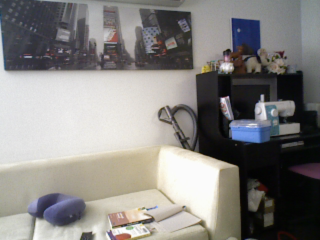
\includegraphics[width=1.5in]{{images/experiments/test_data/Apartment.Texture.rotate.0}.png}
\caption{Frame 1}
\end{subfigure}%
\begin{subfigure}[b]{1.5in}
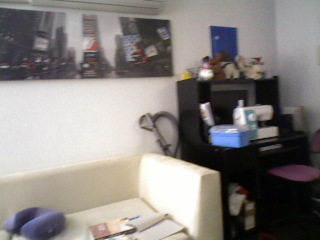
\includegraphics[width=1.5in]{{images/experiments/test_data/Apartment.Texture.rotate.1}.png}
\caption{Frame 10}
\end{subfigure}%
\begin{subfigure}[b]{1.5in}
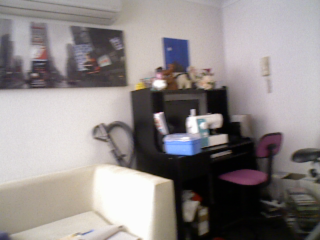
\includegraphics[width=1.5in]{{images/experiments/test_data/Apartment.Texture.rotate.2}.png}
\caption{Frame 15}
\end{subfigure}%
\begin{subfigure}[b]{1.5in}
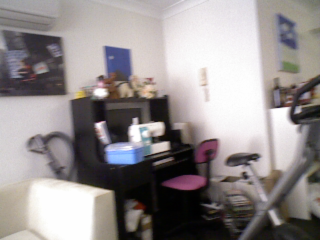
\includegraphics[width=1.5in]{{images/experiments/test_data/Apartment.Texture.rotate.3}.png}
\caption{Frame 20}
\end{subfigure}%
\caption{Apartment.Texture.rotate Scene.}
\label{fig:Apartment_Texture_rotate}
\end{figure*}

